\documentclass[a4paper,12pt]{article}
\usepackage{jae}
\usepackage[dvipsnames]{xcolor}
\usepackage[colorinlistoftodos]{todonotes}
\usepackage{lscape}
\usepackage{longtable}

\newcommand{\Rpkg}[1]{\texttt{#1}}

\title{Navigating through the R packages for movement}
\running{R tracking packages review}

\author{Rocio Joo$^{1*}$ et al.}

\affiliations{
\item Department of Wildlife Ecology and Conservation, Fort Lauderdale Research and Education Center, University of Florida, Fort Lauderdale, FL, USA}

\nwords{XXXX}
\ntables{2}
\nfig{4}
\nref{XX}

\corr{\url{rocio.joo@ufl.edu}}


\begin{document}


\maketitle


\begin{abstract}
  \noindent \begin{enumerate}
  \item The advent of miniaturized biologging devices has provided ecologists with unparalleled opportunities to record animal movement across scales. Technological advancements, including improvements to battery life and data storage, have lead to ever-increasing quantities of data. There have also been concurrent advances in the abundance and sophistication of tools used to process, visualize and analyze biologging data.   
  \item In recent years, there has been greater emphasis on the standardization of methods, but these efforts often occur in parallel, such that there has been a proliferation of programming tools available, but little consensus or advice on their use. Within the R software alone, there are as many as \textcolor{blue}{57} packages for the processing or analysis of tracking data. 
  \item We present a review of these R packages, called here tracking packages, which aims to enable researchers to access the appropriate tools and to provide package developers criteria on what needs to be improved, from a user perspective. Since the packages respond to needs of tools for data processing and analysis, we first divide these aspects into pre-processing, post-processing, data visualization, track description, path reconstruction, behavioral pattern identification, space use characterization, trajectory simulation and others. We describe each of these aspects and, for each of them, we assess which packages offer suitable functionalities and summarize them. 
  \item Supporting documentation is key to render a package accessible to new users. Based on a survey of users, we review the quality of the supporting documentation provided in conjunction with the packages, and identify $12$ packages considered as having good or excellent documentation. 
  \item Compatibility and connectivity between packages is assessed through a network graph analysis. Though a large group of packages has some degree of connectivity (depending on functions or suggesting the use of another tracking package), a third of the packages work on isolation, reflecting a fragmentation in the R movement-ecology programming community. 
  \item At the end of this review, we provide some recommendations to users for choosing packages and to developers for maximizing the usefulness of individual packages and strengthening the links between the programming community. 
  \end{enumerate}
\end{abstract}

\noindent \textbf{Keywords:} biologging, R packages, movement ecology, tracking data



\newpage


\section*{General Introduction}
%
%1. Researchers need to study movement
%2. A systematic way to observe movement is with biologging devices that sample them.
%3. There is a variety of biologging devices, but each comes with pros and cons.
%4. Examples of pros and cons. 
%5. To obtain useful data for analysis, these issues should be solved. Several packages in R (the most used programming language for ecologists) deal with that. 
%6. We will make a list/catalog/road map for packages dealing with each type of biologging device.
%7. Researchers objective is to extract the data from the loggers to later do quantitative analysis. Most of that data ends up in a tracking data format. And many packages are available to analyze that data.
%8. The next section will be about the packages available for data processing and analysis, by stage of analysis. 
%9. This review is for users and developers, because anyone can play both roles. So knowing what exists and what potential gaps there could be, is important for both users and developers. 
%9. Because documentation is key, we did a survey and show results. That way, new users will know which packages are best on that, and developers will have a reference 'scoring' to decide if they will improve their documentation. 
%10. Packages should work together, as people do. So we explore links here. 
%11. Finally, recommendations. 


Animal movement plays a crucial role in ecological and evolutionary processes, from the individual to ecosystem level \textcolor{red}{(Nathan et al. 2008, Kays et al. 2015, other refs)}. However, studying animal movement has presented challenges to researchers, as individuals are often difficult to follow for extended time periods and over large distances. Over recent decades, decreases in the size and cost of animal-borne sensors or biologging devices have led to an exponential increase in their use. This has substantially improved our understanding of how and why animals move \textcolor{red}{(Nathan et al. 2008, other refs)}. Technological advancements have also enabled a wide range of sensors to be used by ecologists, which can be integrated to remotely record a suite of metrics, including x, y and z (i.e. altitude or depth) locations, acceleration, prey capture attempts, as well as in-situ environmental conditions \textcolor{red}{(refs)}. From these multiple sensors, fine-scale behaviors and physiological states can be inferred \textcolor{red}{(Wilmers et al. 2015, other refs)}. 

The increase in quantity and complexity of biologging data requires appropriate analytical and software tools that aid processing and interpretation of data. Those tools should be standardized to allow for reproducibility of results and computation time optimization \textcolor{red}{(Reichman et al. 2011, Stewart Lowndes et al. 2017)}. Mainly in the last decade, many of these tools have been made available for the scientific community in the form of R packages, which has facilitate their widespread use \textcolor{red}{(refs)}. Nonetheless, many packages have been made in isolation, and there is no formal appraisal and comparison of the tools provided by the packages. This limits their use as researchers are required to review each package to identify, within a package, the most appropriate function for their analysis, and between packages with similar objectives, the most appropriate package for their analysis. 
      
The aim of this study is to review the available packages within the R platform, for movement ecology. % I think it's here where I should explain which packages. 
Movement of an organism is defined as a change in the spatial location of an individual in time, so movement data is defined by a space and a time component. For the purpose of this review, we focus on a specific type of movement data: tracking data; i.e. data composed by at least 2-dimensional coordinates $(x,y)$ and a time index $(t)$, and can be seen as the geometric representation (the trajectory) of an individual's path. Since most movement data is collected using tagging devices, some R packages focus on extracting or analyzing data from these devices, dealing with the limitations related to the device they focus on; for instance, some packages provide tools for extracting locations from the light level information collected with Global Location Sensors (GLS). Some other packages have been created to process or analyze any dataset in a tracking data format (x,y,t) regardless of the way the data was collected. All of these packages, that are either for transforming data into a tracking format or to analyze tracking data, are reviewed here and will be henceforth called tracking packages. To our knowledge, there are \textcolor{blue}{$57$} of them. 

The next section will summarize the packages by stage of data processing and analysis (Fig. \ref{fig:DataProcess}). In some cases, biologging devices do not provide raw data in the form of tracking data, e.g. for GLS loggers, for the most part just light intensity is provided. The process by which data is transformed into the (x,y,t) format we refer to as pre-processing. After this, the data may not be immediately usable, e.g. errors or outliers need to be identified, or other second or third order variables need to be derived for the dataset to be ready for analysis; we defined this type of data processing as post-processing. We divide any further analyses into data visualization, track description, path reconstruction, behavioral pattern identification, space use characterization, trajectory simulation and others (e.g. population parameter estimation, interaction between individuals). In each of these subsections, we describe the tools provided by tracking packages to achieve these goals. An additional subsection will briefly describe some R packages that did not deal with tracking data (as defined above), but were developed to process and analyze data from biologging devices such as accelerometers and time-depth recorders. 

\begin{figure}
	\centering
	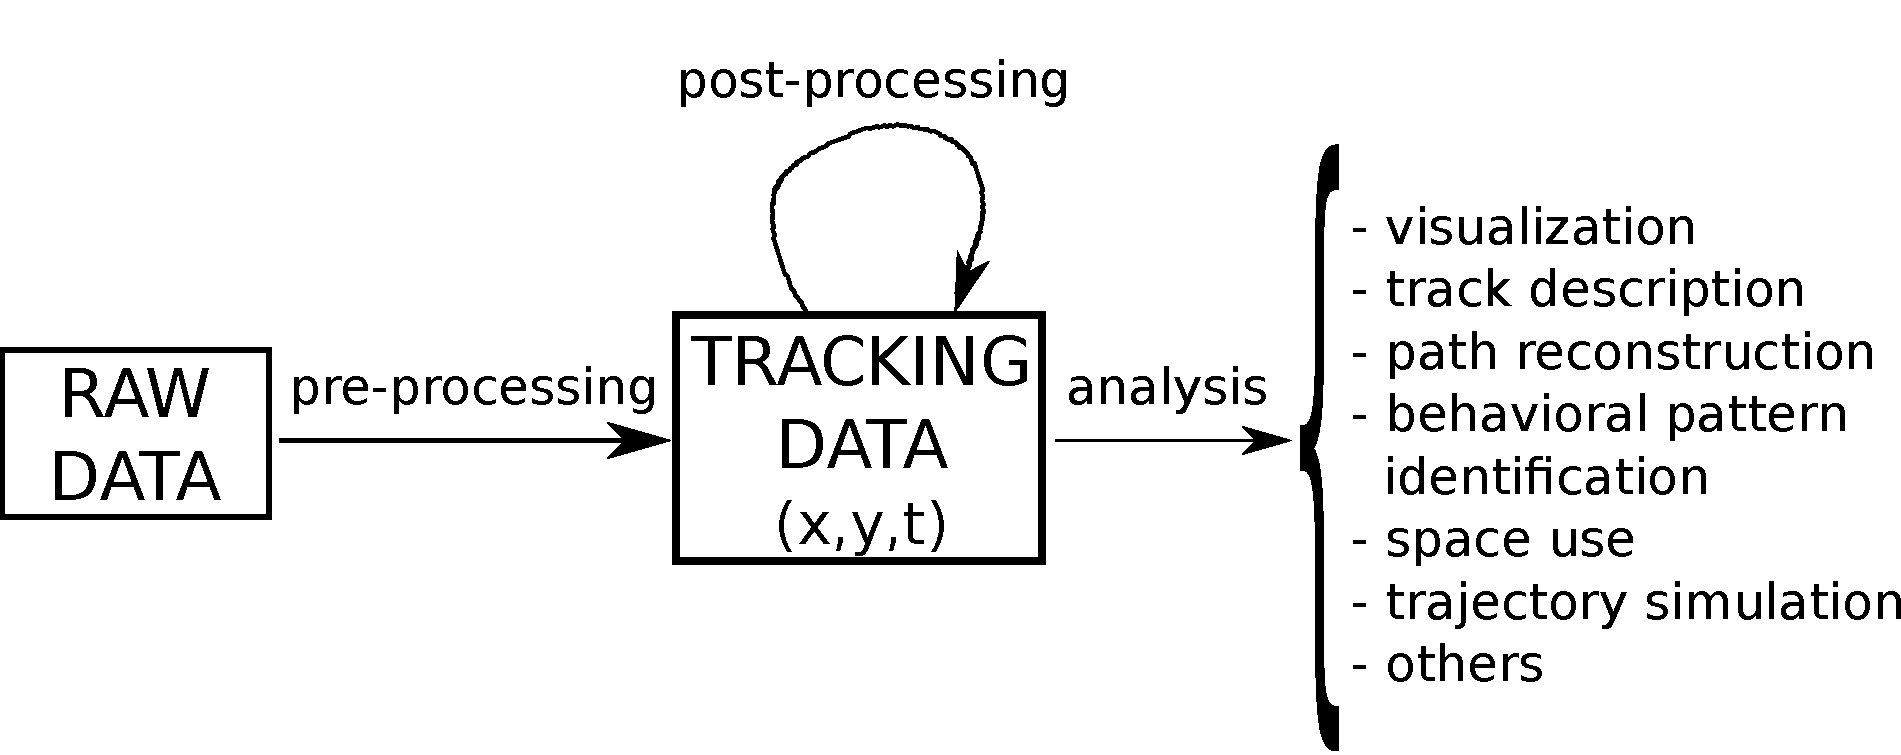
\includegraphics[width=0.75\textwidth]{./mes_images/process-sketch-3.pdf}
	\caption{\label{fig:DataProcess} Stages of data processing and analysis.}
\end{figure} 

Since the documentation provided in conjunction with the packages are key for rendering them accessible, we also review this supporting documentation and, based on a survey, show how useful these documents are to package users. The links between packages, showing how much they rely on each other and the compatibility between them are also assessed. 

This review is aimed at both users and developers of tracking packages, since any user can potentially become a developer at a given time, and any developer can use other packages. This work is a step forward for a complete knowledge on the existing tracking packages; for users, offering criteria to select packages to perform movement ecology analysis, and for developers, discussing issues that could help maximize the usefulness of individual packages and strengthen the links between the community. 


\section*{Data processing, analysis and the R packages}

Multiple sources were used to identify the tracking packages (as defined in the introduction); mainly, 1) the spatio-temporal task view on CRAN (\url{https://cran.r-project.org/web/views/SpatioTemporal.html}, 2) an updated list of this task on GitHub (\url{https://gist.github.com/mdsumner/0a3cb0e58bf9d37b782943ac269e1eff}), 3) packages suggested in the description files of other packages, 4) Google search engine and 5) e-mail/Twitter exchanges with ecologists. The package search was done between March and August 2018. Tracking packages that were either removed from CRAN or described as in a `very early version' on their GitHub repositories were discarded. 

\textcolor{blue}{Fifty seven} packages assist with processing and analysis of tracking data (Fig. \ref{fig:DataProcess}). Some R packages have been developed to tackle several of these stages of data processing and analysis, while others focus on only one. The number of packages regarding each type of processing/analysis is showed in Table \ref{table:PurposeTable}. When appropriate, the type of biologging devices from which the tracking data originates will be described, so that readers that are not familiar with these devices have a basic idea of the advantages and limitations of the devices, and why some packages need to focus on specific issues related to them. 
%
\begin{table}[ht]
	\centering
	\begin{tabular}{lr}
		\hline
		Type of processing/analysis & Count \\ 
		\hline
		Pre-processing & 9 \\
		Post-processing & 17 \\
		Visualization* & 2 \\ 
		Track description & 5 \\ 
		Path reconstruction  & 8 \\ 
		Behavioral patterns identification & 9 \\ 
		Space use & 17 \\ 
		Trajectory simulation & 10 \\ 
		Others & 8 \\ 
		\hline
		Total & 57 \\
		\hline
	\end{tabular}
	\caption{\label{table:PurposeTable} Number of packages dealing with each type of data processing and analysis. Some packages may correspond to more than one category, except for data visualization (*), where only packages created for that purpose are counted.}
\end{table}

The description of packages in this section %(henceforth called `movement packages') 
will also include information on the year each package was publicly available (Fig.\ref{fig:PkgYear}), the main repository where the package is stored and whether it is actively maintained (hereafter referred to as `active'). The official repository for R packages is the Comprehensive R Archive Network (CRAN) repository. CRAN enforces technical consistency, with a set of rules such as the inclusion of ownership information, cross-platform portable code (i.e. to work with Windows, Mac OS and UNIX platforms), minimum and maximum sizes for package components, among others. The great majority of the reviewed packages are on CRAN; the ones that are not on CRAN are mostly on GitHub and a few others are in other repositories (e.g. r-forge or independent websites). Regarding package maintenance, we consider that a GitHub package is actively maintained if a `commit' has been made in the last year, and for the others (if they are not also on GitHub), that the most recent version of the package is no older than one year (analysis conducted in August 2018). Links to each package repository along with a summary of their main characteristics are included in \textcolor{blue}{Supplementary File 1}. 

\begin{figure}
	\centering
	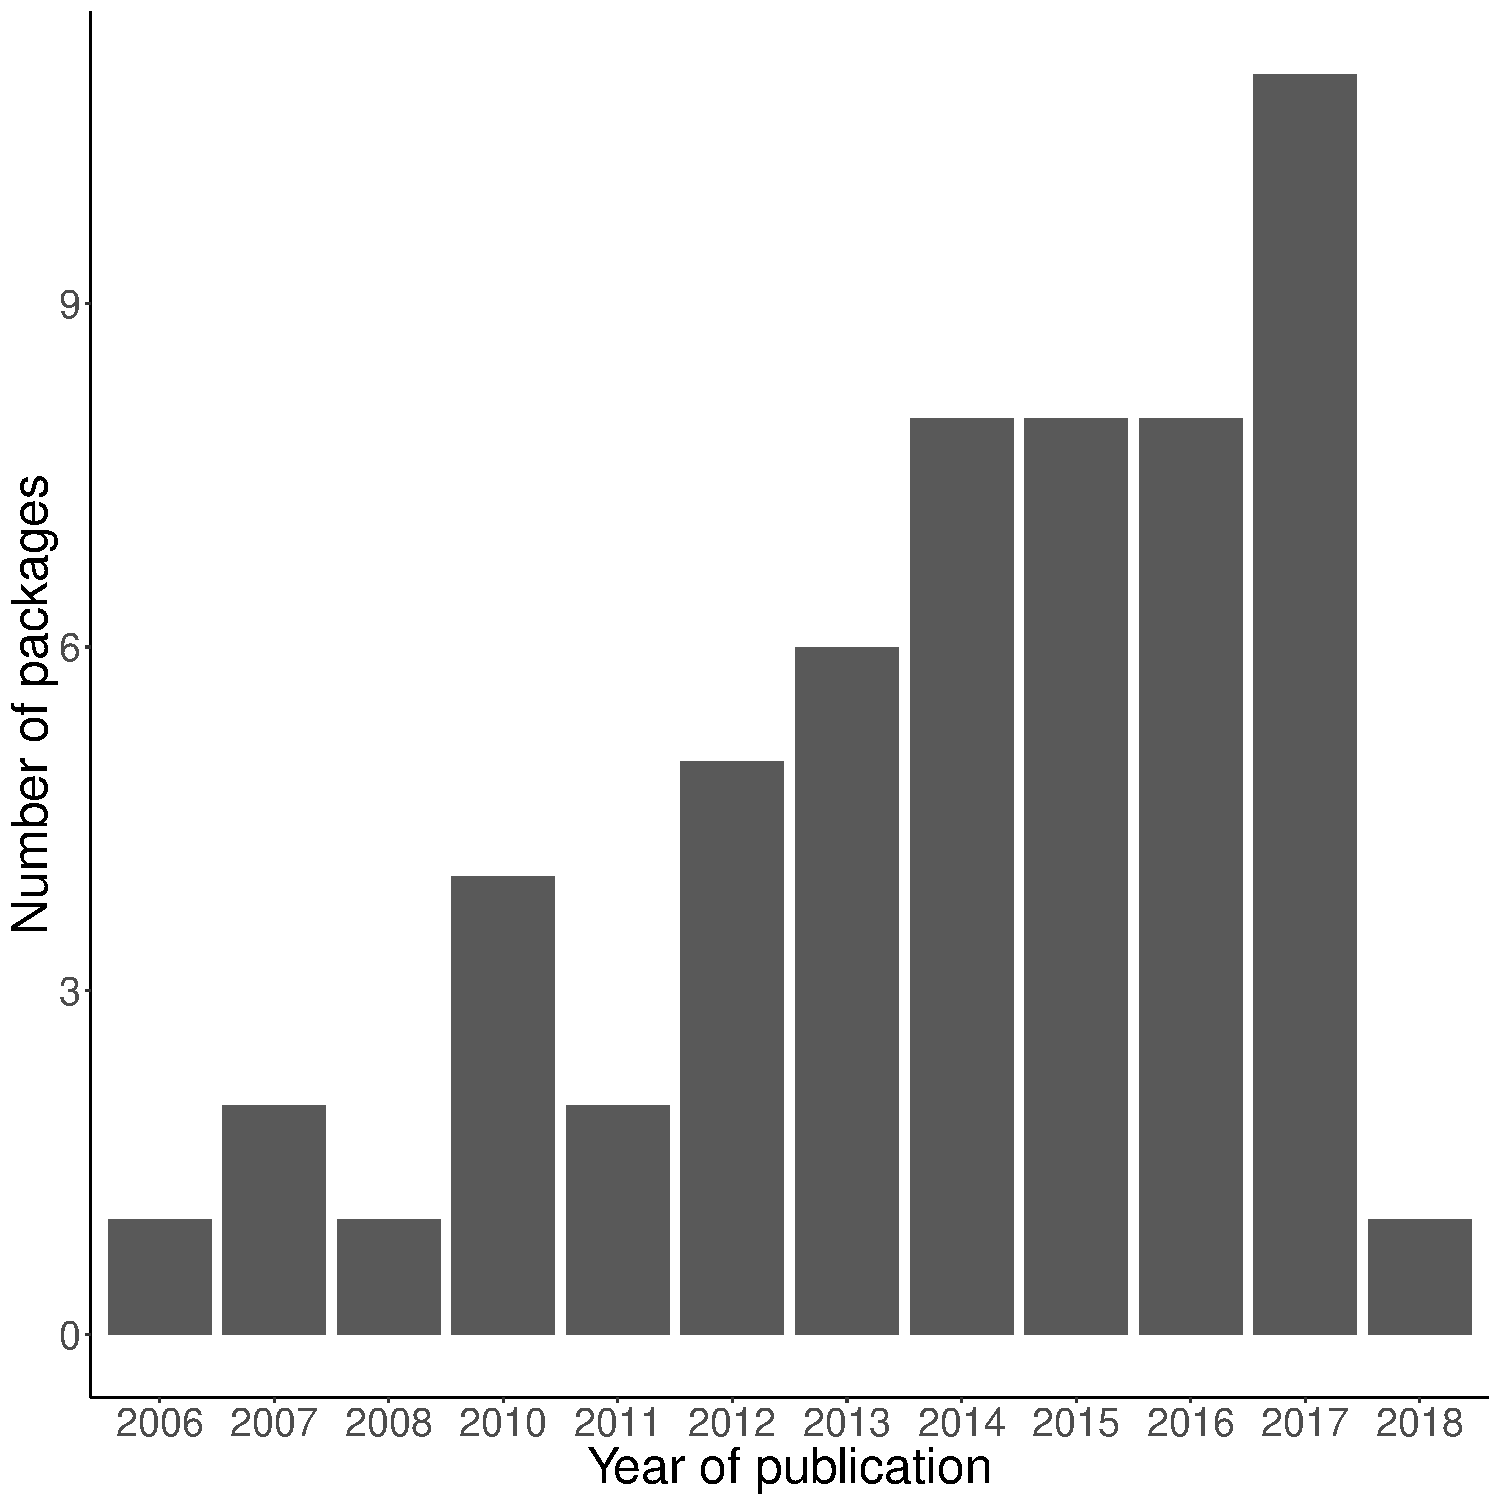
\includegraphics[width=0.75\textwidth]{./mes_images/packages_per_year.pdf}
	\caption{\label{fig:PkgYear} Number of packages per year of publication (assessment performed in August 2018).}
\end{figure} 

\subsection*{Pre-processing} 

When raw biologging data are not in a tracking data format, some pre-processing is required. The methods used for pre-processing depend heavily on the type of biologging device used. Among the tracking packages, \textcolor{blue}{6} are focused on global location sensors (GLS), one on radio telemetry, one uses accelerometry and magnetometry, and another one uses GPS data in addition to accelerometry and magnetometry data. %We will briefly describe the characteristics and challenges of data processing for each type of device and how each package tackles these challenges. % (Table \ref{table:PreDevicesTable}). 
%
%\begin{table}[ht]
%	\centering
%	\begin{tabular}{lr}
%		\hline
%		Type of device & Count \\ 
%		\hline
%		GLS & 6 \\ 
%		Radio & 1 \\ 
%		Acoustic & 1 \\ 
%%		Not biologging & 2 \\
%		Accelerometry, magnetometry and others & 2 \\ 
%		\hline
%		 Total & 11 \\
%		   \hline
%	\end{tabular}
%	\caption{\label{table:PreDevicesTable} Number of packages created for data pre-processing from each type of device.}
%\end{table}

\subsubsection*{GLS data pre-processing} 

GLS are electronic archival tracking devices which record ambient light intensity and elapsed time. The timings of sunset and sunrise are estimated, and latitude is calculated from day length, and longitude from the time of local midday relative to Greenwich Mean time \citep{Afanasyev2004}. GLS can record data for several years and their small size and low mass (<1 g) make them suitable for studying long-distance movements in a wide range of species. Several methodologies have been developed to reduce errors in geographic locations generated from the light data, which is reflected by the large number of packages for pre-processing GLS data. We classified these methods in three categories: threshold, template-fitting and twilight-free.

\begin{itemize}
	\item Threshold methods. Arbitrary threshold levels of solar irradiance are fixed to identify the timing of sunrise and sunset. The packages that use threshold methods are \Rpkg{GeoLight} (2012, CRAN, inactive) and \Rpkg{probGLS} (2016, GitHub, inactive). \Rpkg{GeoLight} uses astronomical equations from \cite{Montenbruck2013} to calculate locations from timings of sunrise and sunset, and from sun elevation angles. \Rpkg{probGLS} implements a probabilistic method that takes into account uncertainty in sun elevation angle and twilight events to estimate locations. Starting with the first known location (where the individual was tagged), it estimates the location of the subsequent twilight event which is replicated several times adding an error term, repeating this process for the whole data series; it then computes probabilities for each location based on the plausibility of the estimated speed or on environmental conditions (e.g. sea surface temperature or SST) \citep{Merkel2016}. 
	\item Template-fitting methods. The observed light irradiance levels for each twilight are modeled in function of theoretical light levels (i.e. the template). Then, parameters from the model (e.g. a slope in a linear regression) are used for estimating the locations. The formulation of the model and the parameters used for location estimation vary from method to method \citep{Ekstrom2004}. The packages that use template-fitting methods are \Rpkg{FLightR} (2015, CRAN, active), \Rpkg{TripEstimation} (2007, GitHub, inactive) and \Rpkg{trackit} (2012, GitHub, active). \Rpkg{FLightR} was particularly developed for bird movement. In its state-space modeling framework \citep{Patterson2008}, the locations are hidden states and the observation model is a physical model of light level changes as a function of position and time. A detailed description of the model and the package functions can be found in \cite{Rakhimberdiev2015} and \cite{Rakhimberdiev2017}, respectively. \Rpkg{trackit} was developed mainly for fish movement. Light intensity around sunrise and sunset are used as inputs in a state-space model that includes solar altitude and SST as covariates \citep{Lam2010}. \Rpkg{TripEstimation} was developed for marine organisms. It uses a Bayesian approach modeling light level as a function of sun elevation at each plausible location, prior knowledge of the animal's movement, and complementary environmental information (e.g. SST, depth of the water column) \citep{Sumner2009}. The package is still available on CRAN, but in its GitHub repository it is indicated that the package was deprecated for \Rpkg{SGAT} (the authors of \Rpkg{TripEstimation} are main authors of \Rpkg{SGAT} and \Rpkg{GeoLight}). \Rpkg{SGAT} contains functions to implement both threshold and template-fitting methods. As one has been deprecated by the other, we consider both packages as one \Rpkg{TripEstimation/SGAT}. As auxiliary packages, \Rpkg{TwGeos} and \Rpkg{BAStag} contain functions to process GLS data such as detecting the timing of twilight periods from light data. The estimated twilight periods can be later used as inputs in the above mentioned packages for location estimation.
	\item Twilight-free methods. It is possible to estimate locations without depending on twilight event identification. %to estimate locations. The packages that fall in this category are \Rpkg{TwilightFree} (2017, GitHub, active), \Rpkg{HMMoce} (2017, CRAN, active). 
	\Rpkg{TwilightFree} (2017, GitHub, active) uses a Hidden Markov Model (HMM) where the hidden states are the daily geographic locations (the spatial domain is discretized as gridded cells) and the observed variable is the observed pattern of light and dark over the day \citep{Bindoff2017}. SST and land/sea marks can be used as covariates. Parameter estimation is performed using functions from the SGAT package. %\Rpkg{HMMoce} is particularly adapted to fish movement and aims at improving location estimation, which implies that locations have been previously obtained by any method (e.g. a GLS provider, or a threshold method) \citep{Braun2017}. It estimates locations via HMMs where the location data are discretized as in \Rpkg{TwilightFree}, and depth-temperature profiles and SST are used as covariates in the observed model. 
\end{itemize}

%\Rpkg{TwGeos} and \Rpkg{BAStag} contain functions to process GLS data such as importing, plotting data and detecting the timing of twilight periods from light data. Depending on the method chosen to estimate locations, those twilight events may be needed. Both  \Rpkg{TwGeos} and \Rpkg{BAStag} were created by the same authors. \Rpkg{BAStag} handles data from British Antarctic Survey (BAS, Cambridge, UK) archival tags, and \Rpkg{TwGeos} was defined by its authors as a `slightly simplified version of \Rpkg{BAStag} with some additional features' (e.g. outlier detection). For that reason, we consider both packages as one.

\subsubsection*{Radio tagging data pre-processing}

Radio tagging involves the attachment of a radio transmitter to an animal. The radio signals transmitted are picked up by an antenna and transformed into a beeping sound by a receiver. As the receiver gets closer to the transmitter, the beeps get louder. Radio tagging can be used to study animal movement by either placing a fixed antenna at a location or through a method called homing, where the researcher moves towards the loudest beeps until the animal has been located. If antennae are located in different locations, triangulation in a map of the direction vectors of the received signals can give an estimate of the animal's location. RFID (radio-frequency identification data) tags can also be used to record when an individual passes through a receiver. With RFID, the researcher does not need to search for beeping signals, but the individual must be adjacent to the receiver to be detected. Radio tags are comparable in price and mass to GLS.  %These are limited as the individual must be adjacent to the receiver, but the tags are very small (XXg) and cheap to purchase. Researchers have to be relatively close to the tagged animals to be able to determine location (necessary proximity could vary between 100 and 500 meters depending on land cover conditions NOT TRUE CAN BE 1km EVEN MORE). 
%

%Two packages implement methods for pre-processing radio tagging data: \Rpkg{telemetr} (2012, GitHub, inactive) and \Rpkg{feedr} (2016, GitHub, active). 
\Rpkg{telemetr} (2012, GitHub, inactive) implements several triangulation methods as well as a maximum likelihood procedure to estimate locations from bearing data (triangulation information). Since there are no reference to the methods in the package documentation, it is aimed at users that are already familiar with the methods.
% \Rpkg{feedr} works with RFID. 

%Three packages focus on radio telemetry for different purposes: \Rpkg{telemetr} (2012, GitHub, inactive) implements location estimation methods, \Rpkg{feedr} (2016, GitHub, active) involves pre-processing of data and obtaining summary statistics and \Rpkg{caribou} (2011, CRAN, inactive) estimates population size based on relocations. A fourth package, \Rpkg{sigloc}, was available on CRAN until June 2018, after which point it was removed.
%
%\begin{itemize}
%	\item \Rpkg{telemetr} implements several triangulation methods as well as a maximum likelihood procedure to estimate locations from bearing data (triangulation information). Since there are no reference to the methods in the package documentation, it is aimed at users that are already familiar with the methods.
%	\item \Rpkg{feedr} works with RFID. RFID use electromagnetic fields to automatically store information of identified animals using radio waves. Raw RFID data typically contains an individual line of data for each read event made by the RFID logger. \Rpkg{feedr} contains functions to read that data, clean it, and most of all, get summary statistics from the data such as number of visits of an animal to static logger stations  and simple movement patterns.
%	\item \Rpkg{caribou} was specifically created to estimate population size from Caribou tracking data and will be described later in the tracking data section.
%\end{itemize}
%
%
%\subsubsection*{Acoustic telemetry}
%%
%Acoustic telemetry uses high frequency sound (between 30 and 300 kHz) to transmit information through water. Tags (transmitters) emit a pulse of sound, which is detected by a hydrophone (or an array of hydrophones) with an acoustic receiver. The distance at which a transmitter can be detected depends on the power and frequency of the tag, and the characteristics of the surrounding environment (e.g. background noise, water turbidity and temperature) \citep{Decelles2014}. 
%
%The only acoustic-specific package is \Rpkg{VTrack} (2015, CRAN, active). \Rpkg{VTrack} was created to deal with VEMCO\copyright (a tagging equipment provider) data, but it can be used with other tracking data set that has a similar data structure to RFID: transmitter ID, receiver ID, datetime stamps, location of receivers. The package contains functions to read the data and get various summary statistics, such as the number of detections per station, observations per individual, or time passed by an individual close to a given station. 
%

\subsubsection*{Accelerometry, magnetometry and GPS data pre-processing} 

Magnetometers measure magnetic fields. Accelerometers measure non-gravitational acceleration, quantifying movement through time by way of changes in velocity. Acceleration is used by ecologists to measure three dimensional movement to classify behaviors such as flight and prey capture, and estimate overall dynamic body acceleration, a measure of energy expenditure. A combined use of magnetometer and accelerometer data (and optionally, other sensors such as gyroscopes) allow obtaining tracks using dead-reckoning (DR) \citep{Wilson2007,Bidder2015,Williams2017}. Typically, data from magnetometers and accelerometers are used to calculate travel vectors (i.e. vectors representing distance covered and direction) for each given time interval, and, since the initial tagging point is known, the three dimensional movement path can be reconstructed by integrating the vectors in sequence. \Rpkg{animalTrack} (2013, CRAN, inactive) and \Rpkg{TrackReconstruction} (2014, CRAN, inactive) implement DR to obtain tracks.

When GPS data are available, \Rpkg{TrackReconstruction} takes DR outputs and forces them to go through known GPS points via space transformation. 
GPS loggers are perhaps the most widely used type of biologging device. They are very cheap and easy to obtain, and location information can be downloaded directly without any post processing. GPS receivers collect but do not transmit information, and infer their own location based on the location of GPS satellites and the time of transmission. Four or more satellites should be visible by the receiver to obtain an accurate result ($<100$ m). GPS receivers can collect precise location data at short time intervals (in the order of minutes or seconds). Combined use of DR and GPS data allows obtaining very high resolution tracking data. 

\subsection*{Post-processing}

Post-processing of tracking data comprises data cleaning (e.g. identification of outliers or errors), compressing (i.e. reducing data resolution which is sometimes called resampling) and computation of metrics based on tracking data, which are useful for posterior analyses.

\subsubsection*{Data cleaning}

\Rpkg{argosfilter} (2007, CRAN, inactive) and \Rpkg{SDLfilter} (2014, CRAN, active) implement functions to filter implausible platform terminal transmitter (PTT) data. Platform terminal (or Argos) transmitters send signals to polar-orbital Argos satellites, which geographically locate the source of the data. They preserve battery life by only needing to transmit signals, leading them to be used for tracking of large-scale migrations, particularly marine mammals and turtles. When the tracked animals are under water, the chances of a satellite receiving PTT signals decrease, so fewer locations can be estimated, and they are likely estimated with fewer satellites, so their accuracy also diminishes. PTTs are particularly useful for individuals that cannot be recaptured, and hence a device recovered. Along with locations, Argos provide accuracy classes (1, 2, 3, 0, A, B, Z) which are associated with different degrees of spatial error \citep{Costa2010}. \Rpkg{argosfilter}'s algorithm is described in \cite{Freitas2007}. It essentially removes records where a location was not estimated as well as locations that required unrealistic travel speeds. SDLfilter, which can also handle GPS data, allow the removal of duplicates, locations estimated with a low number of satellites, biologically unrealistic locations based on speed thresholds or turning angles and locations above high tide lines. The filtering methods are described in \cite{Shimada2012,Shimada2016}.

Other packages with functions for cleaning tracking data are \Rpkg{T-LoCoH} (2013, R-forge, active), \Rpkg{ctmm} (2015, CRAN, active), \Rpkg{TrajDataMining} (2017, CRAN, active) and \Rpkg{trip} (2006, CRAN, active). 

\subsubsection*{Data compression}

Concerning data compression, rediscretization (equal step lengths) can be achieved with \Rpkg{adehabitatLT} (2010, CRAN, active), \Rpkg{trajectories} (2014, CRAN, active) or \Rpkg{trajr} (2018, CRAN, active). Regular time-step interpolation can be performed using \Rpkg{adehabitatLT}, \Rpkg{trajectories} or \Rpkg{amt} (2016, CRAN, active). Other compression methods include Douglas-Peucker (\Rpkg{trajectories} and \Rpkg{TrajDataMining}), opening window (\Rpkg{TrajDataMining}) or Savitzky-Golay (\Rpkg{trajr}). For a brief review on compression methods, see \cite{Meratnia2004}.

\Rpkg{rsMove} (2017, CRAN, active) provides functions to explore and transform tracking data for a posterior linkage with remote sensing data. Location fixes are transformed into pixels and grouped into regions. The spatial or temporal resolution of the tracking data can be changed to match the resolution of the remote sensing data. 

\subsubsection*{Computation of metrics}

Some packages automatically derive second or third order movement variables (e.g. distance and angles between consecutive fixes) when transforming the tracking data into the package's data-class (most packages define their own data classes, see \textcolor{blue}{Supplementary File 1}). These packages are \Rpkg{adehabitatLT}, \Rpkg{trajectories}, \Rpkg{moveHMM} (2015, CRAN active), \Rpkg{momentuHMM} (2017, CRAN, active) and \Rpkg{rhr} (2014, GitHub, inactive). \Rpkg{trip}, \Rpkg{amt}, \Rpkg{trajr} and \Rpkg{move} (2012, CRAN, active) also contain functions for computing those metrics, but the user needs to specify which metric they need to compute. 

\Rpkg{feedr} (2016, GitHub, active) works specifically with RFID data (described above in the radio telemetry subsection). Raw RFID data typically contain an individual line of data for each read event made by each RFID logger. \Rpkg{feedr} contains functions to read raw data from several RFID loggers, and to transform the data of logger detection into movement data for each individual, computing statistics such as the time of arrival and departure from each logger station, and how much time was spent near a station at each visitation. 

\Rpkg{VTrack} (2015, CRAN, active) handles acoustic telemetry data. Acoustic telemetry uses high frequency sound (between 30 and 300 kHz) to transmit information through water. Tags (transmitters) emit a pulse of sound, which is detected by a hydrophone (or an array of hydrophones) with an acoustic receiver. The distance at which a transmitter can be detected depends on the power and frequency of the tag, and the characteristics of the surrounding environment (e.g. background noise, water turbidity and temperature) \citep{Decelles2014}. \Rpkg{VTrack} was created to deal with VEMCO\copyright  (a tagging equipment provider) data, which has a similar structure than RFID; it is composed of transmitter ID, receiver ID, datetime stamps, location of receivers information. Like \Rpkg{feedr} for RFID, \Rpkg{VTrack} can compute statistics such as the time of arrival and departure from each receiver, and how much time was spent near a receiver at each visitation.

\subsection*{Visualization}

Most of the tracking packages contain functions to visualize the data they analyze and we encourage users to explore these functions. 
In this section, we focus on the packages mainly developed for visualization purposes. Those are \Rpkg{anipaths} (2017, CRAN, active) and \Rpkg{moveVis} (2017, CRAN, active). 

They were both conceived for producing animations of tracks. \Rpkg{anipaths} relies on the \Rpkg{animation} package. Users can specify time-steps and seconds per frame for animation, add a background map (e.g. Google Maps) and an individual-level covariate (e.g. migrant, stationary), among others. Consecutive fixes are joined via a spline-based interpolation and a confidence interval for the interpolation of the path for animation can be shown. 

\Rpkg{moveVis} is based on a \Rpkg{ggplot2} plotting architecture and works with \Rpkg{move}-class objects. Users can choose between `true time' which displays the animation respecting the timestamps provided, or `simple' animations where time is not taken into account and all individuals are displayed together as if their tracks started at time 0. Consecutive fixes are joined via linear interpolation. As in \Rpkg{anipaths}, users can specify the number of frames per second and personalize the background map. Statistics related to the background layer (e.g. temperature, land cover) can also be shown as animated lines or bar plots. 

For both packages, animations can be saved in many different formats such as mpeg, mp4 and gif. 

\subsection*{Track description}

\Rpkg{amt}, \Rpkg{movementAnalysis} (2013, GitHub, inactive) and \Rpkg{trajr} compute summary metrics of tracks, such as total distance covered, straightness index, sinuosity and others related to net squared displacement. It should be noted that \Rpkg{movementAnalysis} depends on the \Rpkg{adehabitat} package, was which was officially removed from CRAN in 2018, as it was superseeded by \Rpkg{adehabitatLT}, \Rpkg{adehabitatHR}, \Rpkg{adehabitatHS} and \Rpkg{adehabitatMA} in 2010. \Rpkg{marcher} (2017, CRAN, active), which is focused on migration analysis, also computes net squared displacement as well as a range shift index; i.e. the ratio of the distance between successive circular ranges and their diameter. 

\Rpkg{trackeR} (2015, CRAN, active), which was created to analyze running, cycling and swimming data from GPS-tracking devices for humans, computes metrics summarizing movement effort during each track (or workout effort per session). Those metrics include total distance covered, total duration, time spent moving, work to rest ratio, averages of speed, pace and heart rate. The functionality of this package could be adapted to non-human tracking data.


\subsection*{Path reconstruction}

%Since we defined pre-processing as the stage where raw biologging data is transformed to tracking data (when necessary), path reconstruction is defined here as 
Whether it is for correcting for sampling errors, obtain finer data resolutions or regular time steps, path reconstruction is a common goal in movement analysis. Here we mention methods available, however, before choosing a method, users should be aware that every method is constructed under unique movement assumptions (either inherent to the mathematical model or constructed for a particular species or type of data), and users should refer to the literature on the methods first. Packages available for path reconstruction are \Rpkg{HMMoce} (2017, CRAN, active), \Rpkg{kftrack} (2011, GitHub, active), \Rpkg{ukfsst/kfsst} (2012, GitHub, active), \Rpkg{bsam} (2016, CRAN, active), \Rpkg{argosTrack} (2014, GitHub, active), \Rpkg{BayesianAnimalTracker} (2014, CRAN, inactive), \Rpkg{crawl} (2008, CRAN, active) and \Rpkg{ctmcmove} (2015, CRAN, active). While the first three are focused on GLS data, \Rpkg{bsam} is intended for PTT data, \Rpkg{BayesianAnimalTracker} combines GPS data and dead-reckoning, and the other two could be used with any tracking data.

\subsubsection*{Improving location estimation from GLS data}

\Rpkg{kftrack}, \Rpkg{kfsst} and \Rpkg{ukfsst} were developed by the same team of \Rpkg{trackit}, described in the pre-processing section. As \Rpkg{trackit}, they are mainly focused on fish movement. \Rpkg{kftrack}, \Rpkg{ukfsst} and \Rpkg{kfsst} use already estimated positions, either by the threshold method or given by the provider, and improve those estimations using a 2-dimensional random walk model \citep{Sibert2003}. Because of the generality of this modeling framework, \Rpkg{kftrack} could actually be used for any tracking data. In addition to the random walk model, \Rpkg{kfsst} includes SST as a covariate in the model \citep{Nielsen2006}, but it has been superseded by \Rpkg{ukfsst}, which implements an optimized parameter estimation. For that reason, we count \Rpkg{kfsst} and \Rpkg{ukfsst} as one.

\Rpkg{HMMoce}, also adapted to fish movement and working with already estimated/provided locations, uses HMMs (like \Rpkg{TwilightFree}) and incorporates depth-temperature profiles and SST as covariates in the observed model \citep{Braun2017}. 

\subsubsection*{Improving location estimation from PTT data}

\Rpkg{bsam} estimates locations by fitting Bayesian state-space models to the data. They offer possibility of accounting for different movement patterns using `switching' or HMMs; if this is opted out, first-difference correlated random walk models (DCRWs) are used. It is possible to estimate some of the model parameters for each individual and others at the population level (see \cite{Jonsen2013,Jonsen2016} for more details). The \Rpkg{argosTrack} package fits several types of movement models to PTT data \citep{Albertsen2015}, such as correlated random walks (CRWs) in discrete and continuous versions, and Ornstein-Uhlenbeck (OU) models, using Laplace approximation via Template Model Builder. 

\subsubsection*{Combining dead-reckoning and GPS data}

\Rpkg{BayesianAnimalTracker} takes an already estimated DR path and combines it with GPS data via a Bayesian approach \citep{Liu2016}: it maximizes the likelihood of a model where it is assumed that the true points come from a Brownian Bridge, both the GPS and DR points are linearly dependent on the true path, and random and measurement error parameters are added to the model.

\subsubsection*{Modeling movement of general tracking data}

\Rpkg{crawl} reconstructs paths by fitting continuous-time CRW models (called CTCRWs) \citep{Johnson2008} to tracking data. Though it can be used for any tracking data, \Rpkg{crawl} can account for the accuracy classes of PTT data to model the error in location. \Rpkg{ctmcmove} fits a functional movement model \citep{Buderman2016} to the data and a set of probable true paths can be generated. 

\subsection*{Behavioral pattern identification}

Another common goal in movement ecology is to get a proxy of the individual's behavior through the observed movement patterns, based on either the locations themselves or second/third order variables such as distance, speed or turning angles. Covariates, mainly related to the environment, are frequently used for behavioral pattern identification. 

We classify the methods in this section as: 1) non-sequential classification or clustering techniques, 2) segmentation and 3) hidden Markov models.

\subsubsection*{Non-sequential classification or clustering techniques}

Each fix in the track is classified as a given type of behavior, independently of the classification of the preceding or following fixes. \Rpkg{EMbC} (2015, CRAN, active) and \Rpkg{m2b} (2017, CRAN, inactive) present tools that fall in the first category. \Rpkg{EMbC} implements the Expectation-maximization binary clustering method \citep{Garriga2016}. \Rpkg{m2b} implements a random forest (a wrapper for the \Rpkg{randomForest} package functions) to classify behaviors using a supervised training dataset, thus a dataset of both tracking data and known behaviors is needed to train the model.

\subsubsection*{Segmentation methods}

A time series of movement patterns is cut into several segments; the edges of each segment represent a change in behavior. \Rpkg{adehabitatLT}, \Rpkg{bcpa} (2013, CRAN, inactive), \Rpkg{marcher} and \Rpkg{migrateR} (2016, GitHub, active) implement segmentation methods. \Rpkg{adehabitatLT} presents two of these methods: Gueguen and Lavielle. \Rpkg{bcpa} implements the behavioral change point analysis \citep{Gurarie2009}. Both \Rpkg{marcher} and \Rpkg{migrateR} are suited for migrant individuals. \Rpkg{marcher} enables a mechanistic range shift analysis \citep{Gurarie2017} that identifies changes in locations of focal ranges, so migration and resident behaviors can be distinguished. The ranging models available in the package can take into account autocorrelation in location and in velocity. \Rpkg{migrateR} uses net displacement models to identify migrant, resident and nomad behavior \citep{Spitz2017}. The models can incorporate factors such as elevation, sensitivity to starting date in the series, minimum time out of residence zone, among other features.  

\subsubsection*{Hidden Markov models}

The main idea is that there is a hidden state process (representing the sequence of non-observed behaviors) conditioning the observed movement patterns, and that the states follow a Markov process \citep{Langrock2012}. In this category we consider standard as well as more complex versions of these models; e.g. adding hierarchical structures, a second observation process for locations (state-space modeling), covariates affecting different components in the model, autoregressive processes or a spatial covariance structure. \Rpkg{bsam}, \Rpkg{moveHMM} and \Rpkg{momentuHMM} implement methods that fall in the HMM category. \Rpkg{bsam}, for PTT data, implements Bayesian state-space models as described in the path reconstruction section, and may incorporate a layer of two switching states into the model: one state representing directed fast movement, and the other representing relatively undirected slow movement \citep{Jonsen2013}. \Rpkg{moveHMM} and \Rpkg{momentuHMM} are not restricted to two states. \Rpkg{moveHMM} implements HMMs incorporating covariates and allowing for state sequence reconstruction, i.e. sequences of the behavioral proxies, via the Viterbi algorithm. In \Rpkg{moveHMM}, the variables modeled in the observed process are step length and turning angles, or two variables that statistically behave as step length and turning angles. \Rpkg{momentuHMM} implements generalized Hidden Markov models \citep{McClintock2012} with great flexibility for the choice of observed variables and their probability distributions, and covariate incorporation in the models. Since HMMs require regular time steps, \Rpkg{momentuHMM} offers a multiple imputation method \citep{McClintock2017}: it fits a CTCRW (from \Rpkg{crawl}) to the data obtaining regular time-step realizations and then fits an HMM to those realizations; all of this is done multiple times. Even if the data classes and model formulation in the package differ from \Rpkg{moveHMM}, many of the HMM-related functions are based on \Rpkg{moveHMM}. \Rpkg{moveHMM} is more user-friendly than \Rpkg{momentuHMM}, but \Rpkg{momentuHMM} offers greater modeling possibilities. 

\subsection*{Space and habitat use characterization}

Spatial ecology precedes movement ecology as a research field, which is why a main interest in movement ecology is to use tracking data to answer questions related to space and habitat use, such as: where do individuals spend their time, how long do they stay in different places and what role environmental conditions play in these choices? Multiple packages implement functions to help answering these questions, which are typically split into two categories: home range calculation and habitat selection.

\subsubsection*{Home range}

Several packages allow the estimation of home ranges: \Rpkg{adehabitatHR} (2010, CRAN, active), \Rpkg{rhr}, \Rpkg{T-LoCoH}, \Rpkg{BBMM} (2010, CRAN, inactive), \Rpkg{mkde} (2014, CRAN, inactive), \Rpkg{MovementAnalysis} and \Rpkg{move}. They provide a variety of methods, from simple Minimum convex polygons (MCP) \citep{Mohr1947} to more complex probabilistic Utilization distributions (UD) \citep{VanWinkle1975}, potentially accounting for the temporal autocorrelation in tracking data, as detailed below.

\begin{itemize}
	\item \Rpkg{adehabitatHR} contains a comprehensive list of methods to estimate home ranges: convex hull methods like MCP, clustering techniques, Local convex hulls (LoCoH) \citep{Getz2007} and the characteristic hull method \cite{Downs2009}; UD methods like kernel home ranges, also with the modification from \cite{Benhamou2010} to account for boundaries, and methods to account for temporal autocorrelation between locations (Brownian bridge kernel method) \citep{Bullard1991}; biased random bridge kernel method also known as movement-based kernel estimation \citep{Benhamou2010, Benhamou2011}; and product-kernel algorithm, \cite{Horne2007}.
	\item \Rpkg{rhr} \citep{Signer2015} provides a graphical user interface to estimate home ranges using several non-movement based methods, such as parametric home ranges, MCP, kernel UD, or local convex hulls, as well as the Brownian Bridge kernel method (as a wrapper to the \Rpkg{adehabitatHR} function). Complementary analyses include time to statistical independence, site fidelity test (against random permutation of step lengths and angles), among others.
	\item \Rpkg{T-LoCoH} is focused on constructing home-range hulls \citep{Lyons2013}. A time-scale distance metric and a set of different nearest-neighbor criteria are available to choose which points to consider in a same hull. Hull metrics for space use, such as number of revisitations (repeated visits of an individual to the same hull) and their durations are also computed. Although the package was originally implemented for GPS data, it can be used for tracking data in general. 
	\item \Rpkg{BBMM}, \Rpkg{MovementAnalysis} and \Rpkg{mkde} use Brownian bridge movement models to obtain UDs. \Rpkg{mkde} allows for a 3D extension of the Brownian bridges \citep{Tracey2014}.
	\item \Rpkg{move}, in turn, calculates UDs of tracking data via dynamic Brownian Bridge modeling \citep{Kranstauber2012} or uses MCP for home range estimation; for the latter, it imports functions from \Rpkg{adehabitatHR}.
\end{itemize}

\subsubsection*{Habitat use}

The role of habitat features on animal space use, or habitat selection, can be investigated with any of the following four packages. 

\begin{itemize}
	\item \Rpkg{adehabitatHS} (2010, CRAN, active) provides several tools for exploratory habitat selection analysis, from simple univariate analyses, such as resource selection ratios \citep{Manly2007} or compositional analysis \citep{Aebischer1993}, to a family of multivariate analyses based on the geometric concept of ecological niche \citep{Hutchinson1957}, or the Outlying Mean Index (OMI) \citep{Doledec2000} and the K-select \citep{Calenge2005} at the individual level.
	\item \Rpkg{hab} (2015, GitHub, inactive) enhances several utility functions of \Rpkg{adehabitatHS}, \Rpkg{adehabitatHR} and \Rpkg{adehabitatLT}, and provides core functions to prepare, fit and evaluate Step Selection Functions (SSFs) \citep{Fortin2005} while relying on \Rpkg{adehabitatLT} classes to handle trajectories. SSFs essentially investigate habitat selection along the trajectory, by comparing habitat features at observed step locations with those at alternative random steps taken from the same starting point \citep{Thurfjell2014}.
	\item \Rpkg{amt} contains functions and wrappers to streamline the process of fitting SSFs from pairs of coordinates defining locations, to the conditional logistic regression model.
	\item In \Rpkg{ctmcmove}, the role of habitat features is investigated through a generalized linear model framework, for which these features are rasterized, and the animal track is first imputed via functional movement modeling and then discretized in a grilled space (more details in \cite{Hanks2015}). 
\end{itemize}

\subsubsection*{Non-conventional approaches for space use}

Other non-conventional approaches for investigating space use from tracking data can be found in \Rpkg{ctmm}, \Rpkg{moveNT} (2017, GitHub, active), \Rpkg{recurse} (2017, CRAN, active), \Rpkg{rsMove}, \Rpkg{feedr} and \Rpkg{VTrack}. 

\begin{itemize}
	\item \Rpkg{ctmm} fits several candidate movement models via a variogram regression approach \citep{Fleming2014}; those models can account for spatial autocorrelation in locations and periodicity in space use if required \citep{Peron2016}. Space utilization is computed via an autocorrelated kernel estimator, where the autocorrelation term comes from the movement model previously fitted \citep{Fleming2015}. 
	\item \Rpkg{moveNT} tackles space use analysis via network graph theory \citep{Bastille2018}. We summarize the procedure here: 1) Tracking data is represented over a gridded map and the number of transitions between pixels are counted. 2) The adjacency matrix, i.e. the counts of transitions, are then used to compute some network metrics at the pixel level. 3) A Gaussian mixture model is fitted to one of the metrics (user choice) to cluster values in two groups potentially representing patches and interpatch movement.
	\item \Rpkg{rsMove} implements a procedure to identify feeding sites from tracking data as a function of environmental variables (remote sensing data). It uses a random forest classification model; however, there is no information about how to fix the parameters of the model, so users should be careful when using this method. An application of the method can be found in \cite{Remelgado2017}, but the parametrization is not described in the manuscript.
	\item \Rpkg{recurse} aims at computing number of revisitations to pre-defined areas and their duration. These areas can be defined by the user by entering their center of gravity (by default, the fixes in the track) and a radius. The vignette gives important criteria to use the functions and interpret the results, though there are no citations of scientific publications.
	\Rpkg{feedr} and \Rpkg{VTrack}, for radio and acoustic telemetry data, respectively, provide statistics on animal visits to given logger stations/receivers. 
	% * <basille@ufl.edu> 2018-09-11T14:14:38.538Z:
	% 
	% > The vignette gives important criteria to use the functions and interpret the results.
	% No reference literature for this approach? Seems similar to residence time vs. time to return in Van Moorter et al. (2016), which is based on the idea of recursion.
	% 
	% - Van Moorter, B., Rolandsen, C. M., Basille, M., & Gaillard,
	%   J. (2016). Movement is the glue connecting home ranges and habitat
	%   selection. Journal of Animal Ecology, 85(1),
	%   21–31. http://dx.doi.org/10.1111/1365-2656.12394
\end{itemize}

\subsection*{Trajectory simulation} 

Simulating trajectories can be useful to test hypotheses concerning movement, by comparing the patterns of simulated movement from several alternative theoretical models, or the patterns in the simulated movement to those of real observed tracks. In addition, simulation allows the quantification of estimator uncertainty by parametric bootstrapping (e.g. \cite{Michelot2016}). As with other types of data analysis, simulations highly depend on the model used by the researcher. 
The tracking packages implement trajectory simulation mainly based on Hidden Markov models, correlated random walks, Brownian motions, L\'evy walks or Ornstein-Uhlenbeck processes. %For more on movement models, readers can refer to Codling et al. 2008, McClinctock et al. 2014 or Patterson et al. 2017.

Packages that allow simulation of trajectories from movement models fitted to tracking data are \Rpkg{moveHMM}, \Rpkg{momentuHMM} (HMMs), \Rpkg{bsam} (DCRWs), \Rpkg{crawl} (CTCRWs), \Rpkg{argosTrack} (discrete and continuous CRWs, and OU processes) and \Rpkg{ctmm} (several continuous time movement models). These packages have been described in the previous sections, and the simulations are presented as additional features after model fitting in their documentation. Another package for model fitting and simulation is \Rpkg{smam} (2013, CRAN, inactive). It can fit and simulate two types of movement models: Brownian motions with measurement error \citep{Pozdnyakov2014} and moving-resting processes with Brownian motion for the moving stage \citep{Yan2014}.

Other packages implemented simulation functions when movement parameters are known; i.e. there is no previous fitting to tracking data. \Rpkg{adehabitatLT} proposes trajectory simulation using Brownian motion-based models, L\'evy walks, CRWs and bivariate OU motion. \Rpkg{trajr} allows for CRWs, directed random walks (direction is equal to a constant plus a small noise), Brownian motion and L\'evy walks. \Rpkg{moveNT} enables simulation of movement within and between patches. Movement within patches can follow an OU process (wrapping functions from \Rpkg{adehabitatLT}) or a two-states movement model (wrapping functions from \Rpkg{moveHMM}). Movement between patches is simulated via a Brownian bridge movement model (from \Rpkg{adehabitatLT}). 

\Rpkg{SiMRiv} (2016, CRAN, active) is another package created for simulation and it can take into account environmental constraints. It allows simulating random walks, correlated random walks, multi-state movement and constraining the area by an environmental resistance variable -- defined by the user -- that conditions the direction of the movement. The available documentation gives a detailed explanation of the simulation process. 

\subsection*{Other analyses of tracking data}

\subsubsection*{Interactions}

Interactions between individuals can be assessed using metrics from \Rpkg{wildlifeDI} (2014, CRAN, active), which quantifies the dynamic interaction between two tracks of distinct individuals through several metrics (see \cite{Long2014} for details). The package relies on ltraj objects (the \Rpkg{adehabitatLT} data class). Other packages that include functions investigating interaction are \Rpkg{TrajDataMining} and \Rpkg{movementAnalysis}: \Rpkg{TrajDataMining} can identify potential partners based on distance and time thresholds fixed by the user and \Rpkg{MovementAnalysis} computes the expected duration of encounters at each location for every pair of IDs, based on a Brownian Bridge movement model fitted to the tracking data. 

\subsubsection*{Movement similarity}

\Rpkg{SimilarityMeasures} (2015, CRAN, inactive) assesses similarity between trajectories using metrics such as the longest common subsequence (LCSS), Fr\'echet distance, edit distance and dynamic time warping (DTW). Curious readers can refer to \cite{Magdy2015} for a brief review on trajectory similarity measures. \Rpkg{trajectories} also computes the Fr\'echet distance for two trajectories. 

\subsubsection*{Population size}

\Rpkg{caribou} (2011, CRAN, inactive) was specifically created to estimate population size from Caribou tracking data, but can also be used for wildlife populations with similar home-range behavior. The methods implemented here are described in \cite{Rivest1998}. The user needs to specify parameters concerning the size of each detected group, the number of collars in each of these groups and the detection model to use. 

\subsubsection*{Inferring environmental variables from tracking data}

Using tracking data to infer an environmental variable is the objective of \Rpkg{moveWindSpeed} (2016, CRAN, active). It uses bird tracking data to estimate wind speed via a maximum likelihood approach \citep{Weinzierl2016}. The estimation is only performed for segments where the bird is circling in a thermal, so a function in the package identifies those segments. Speed is modeled as a mean with an autocorrelated drift. 

\subsubsection*{Database management}

Finally, \Rpkg{rpostgisLT} (2016, CRAN, active) handles database management for trajectory data by integrating R and the `PostgreSQL/PostGIS' database system. The package relies on \Rpkg{adehabitatLT}, and allows users to run the analyses on their database that can be usually done with an ltraj object in \Rpkg{adehabitatLT}. 

\subsection*{Analysis of biologging but not tracking data}

Time-depth recorders (TDRs) collect data on depth, velocity and other parameters as animals move through the water. These biologging data by themselves do not allow obtaining tracking data (x,y,t) and thus comparable analyses to the ones presented above. \Rpkg{divemove} and \Rpkg{rbl}, the latter also for accelerometer data, are the two packages implementing TDR data analysis. \Rpkg{divemove} contains functions to identify wet and dry periods in the series, calibrate depth and speed sensor readings, identify individual dives and their phases, summarize statistics per dive and plot the data. With \Rpkg{rbl}, accelerometry data are used for identifying prey catch attempts \citep{Viviant2010} and swimming effort from frequency and magnitude of tail movement \citep{Bras2016}. Other functions allow the extraction of summary statistics from dives (e.g. maximum depth), fitting broken stick models (i.e. piecewise linear regression) to dive series and identifying dive phases. 

Accelerometry data is also used in human studies, primarily to assess levels of physical activity. Six R packages focus on the analysis of human accelerometry data, mainly to describe periodicity and levels of activity. \Rpkg{accelerometry}, \Rpkg{GGIR} and \Rpkg{PhysicalActivity} identify wear and non-wear time of the accelerometers. \Rpkg{nparACT} computes descriptive statistics such as interdaily stability, intradaily variability and relative amplitude of activity \citep{Blume2016}. \Rpkg{acc}, \Rpkg{GGIR} and \Rpkg{pawacc} classify wear data into different levels of activity (e.g. sedentary, moderate and vigorous) using thresholds given by the user, and offer some functions for visual representation of the data and descriptive statistics on the types of activities. Additionally, \Rpkg{acc} allows for activity simulation via Hidden Markov modeling.

The packages described in this section are not tracking packages and will not be discussed in the next sections, but readers should take them into consideration when analyzing TDR and accelerometer data. The packages focused on human data can be used for animal data as well. 

\section*{Packages documentation}
%\label{section:documentation}

Documentation in the form of manuals, vignettes, tutorials or published articles is key to understanding how to use a package's features for the first time, especially if the package contains a large number of functions and tools. %Assessing how helpful the documentation is, and how this is related to the frequency of use or the relevance of a package can be valuable inputs for package maintainers and future package developers. 
Without proper user testing and peer editing, package documentation can lead to large gaps of understanding and lower usefulness for users. If functions and work flows are not expressly defined, a package's capacity to help users is undermined. Vignettes can act as road maps for the user, and published articles expressly pertaining to the package help provide context and guidance on the internal workings of functions. Moreover, since packages make specific methods available for R users, the documentation should not only explain how to use the packages but also explain or provide references for the methods. %Additionally peer-reviewed articles provide convenient supplementary material, and strength package credibility. 
% should be assessed through a survey directed to package users, which is a next stage after this review 
% The function of `readability' and 'useability' from documentation was not systematically assessed for the packages in this review, though for this work many of the packages required significantly more searching and testing time to quantify metrics and describe package function. 

To assess package documentation, an online survey was conducted \textcolor{blue}{between August and October} 2018. Questions in the survey regarded helpfulness of package documentation and the frequency of package use. 
The survey was posted on Twitter and sent to several email lists of ecology and R related groups, and completed by \textcolor{blue}{225} people. The exact formulation of each question in the survey, summarized results and a discussion on the representativity of the survey are shown in \textcolor{blue}{Supplementary File 2 and 3}. %There was no previous selection of the participants and no probabilistic sampling was involved. 
%The packages considered for the survey differ slightly from those considered for this review: \Rpkg{movement} and \Rpkg{sigloc} packages in the survey were not considered here because the former was stated as in a `very early version' by the developers, and the latter was removed from CRAN. Moreover, 
All of the packages in this review were considered in the survey except for \Rpkg{trajr}, which was added to the review after the survey started. 

 % The main question in the survey asked users to evaluate, for each of the packages they have used, the level of helpfulness of the documentation provided. Available options were 1) Not enough: It's not enough to let me know how to do what I need; 2) Basic: It's enough to let me get started with simple use of the functions but not to go further (e.g. use all arguments in the functions, or put extra variables); 3) Good: I did everything I wanted and needed to do with it; 4) Excellent: I ended up doing even more than what I planned because of the excellent information in the documentation; 5) I honestly can't remember. 

We identified \textcolor{blue}{12} packages (for which we had at least 10 respondents) as having `great documentation', meaning that more than $75\%$ of the respondents expressed that the documentation was either good (allowing the user to do everything they wanted and needed to do with the package) or excellent (allowing users to do even more than what they initially planned because of the excellent quality of the information). These are: \Rpkg{momentuHMM} ($93.8\%$), \Rpkg{moveHMM} ($89.5\%$), \Rpkg{adehabitatLT} ($88.6\%$), \Rpkg{adehabitatHS} ($86.1\%$), \Rpkg{adehabitatHR} ($83.1\%$), \Rpkg{EMbC} ($81.8\%$), \Rpkg{wildlifeDI} ($81.3$), \Rpkg{ctmm} ($80.0\%$), \Rpkg{GeoLight} ($76.9\%$), \Rpkg{move} ($76.6\%$), \Rpkg{recurse} ($76.5\%$), and \Rpkg{bsam} ($76.2\%$) (see Fig. \ref{fig:DocParticipants}). From this group of packages, \Rpkg{momentuHMM} and \Rpkg{move} offer manuals and vignettes, while all the others offer in addition scientific articles centered on the package. Also, if we look at the packages used by more than $50$ participants, all except for \Rpkg{crawl} had `great documentation'. % Packages with `great documentation' were also identified as either important or essential for the core work of most of their users (Fig. \ref{fig:DocRelevance}). 

Package developers could use the results of this survey (see \textcolor{blue}{Supplementary File 3} for more details) as a guidance to decide on whether to improve the documentation of their packages so more researchers can use them. 

\begin{figure}
	\centering
	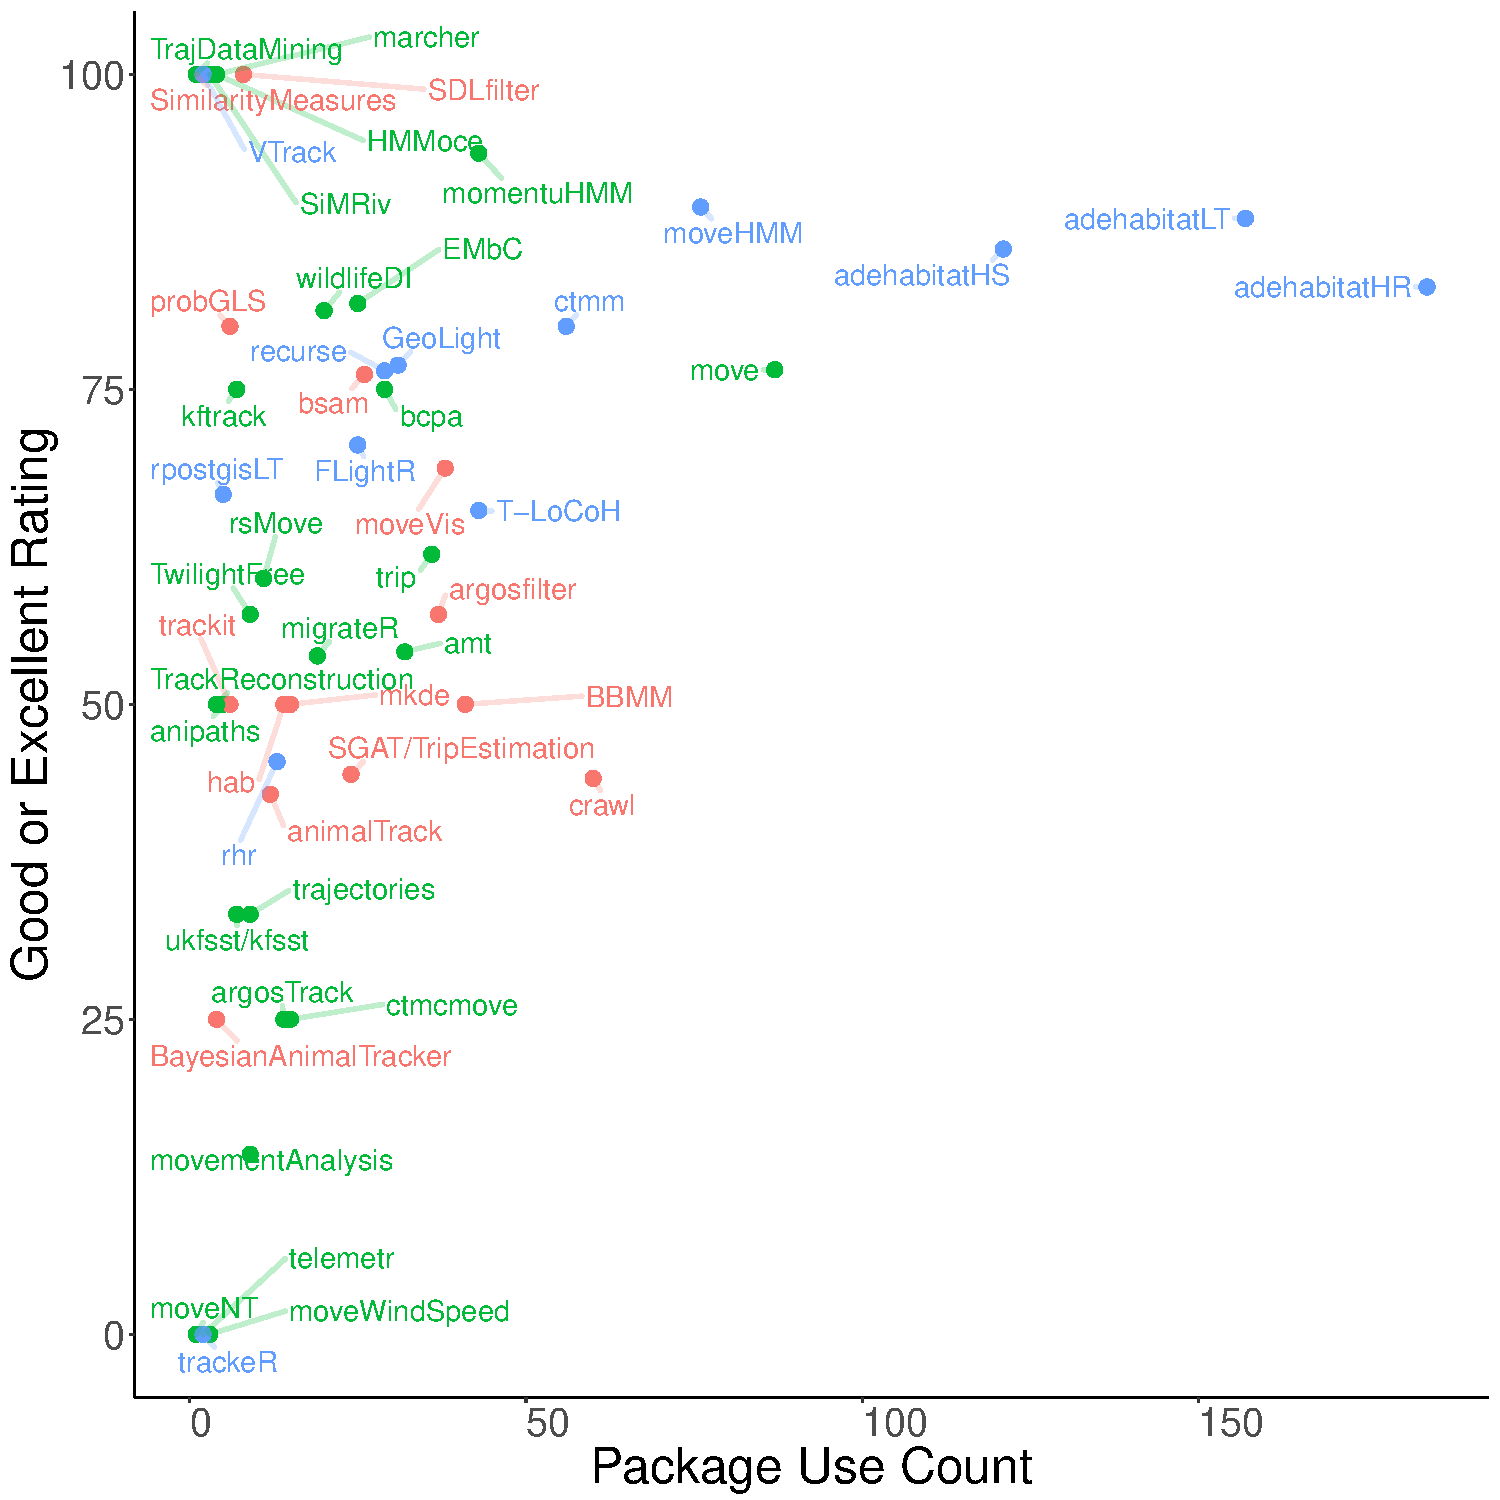
\includegraphics[width=1\textwidth]{./mes_images/doc_vs_participants_noleg.pdf}
	\caption{\label{fig:DocParticipants} Packages with good and excellent documentation (survey results). x axis: Number of survey participants that used each package; y axis: percentage of users of each package that considered the documentation good or excellent. Text color in red corresponds to packages with standard documentation only, green is for packages with vignettes, and blue is for packages that also released other types of documentation.}
\end{figure}

%Due to large differences in the number of responses per package, and for some of packages, the high percentage of users who did not remember characteristics about the documentation, no statistical test was performed, since it could lead to spurious conclusions. We focused instead in the identification of `great-documentation' packages, for which more than $80\%$ of the respondents expressed that the documentation was either good (allowing the user to do everything they wanted and needed to do with the package) or excellent (allowing users to do even more than what they initially planned because of the excellent quality of the information). Ten packages (for which we had at least 10 respondents) corresponded to this category: \Rpkg{EMbC} ($94\%$), \Rpkg{momentuHMM} ($92\%$), \Rpkg{bcpa} ($92\%$), \Rpkg{moveHMM} ($90\%$), \Rpkg{adehabitatLT} ($88\%$), \Rpkg{move} ($86\%$), \Rpkg{adehabitatHS} ($86\%$), \Rpkg{adehabitatHR} ($83\%$), \Rpkg{ctmm} ($82\%$) and \Rpkg{recurse} ($82\%$). We also asked about the relevance of each package for the user's work. All of the great-documentation packages were either important or essential for the core work of more than half of their users.
%
%Moreover, there are some packages that -- based on the survey -- should improve their documentation, such as \Rpkg{BBMM}, \Rpkg{crawl} and \Rpkg{SGAT}. Less than $50\%$ of their users (that replied about documentation in the survey) considered that the documentation was good or excellent. Documentation improvement would be very helpful for \Rpkg{crawl} users since $60\%$ of them declared to consider the package important or essential for the core of their work. 
%
%

\section*{Links between the packages}
\label{section:links}

We analyzed the links between tracking packages. If a package needs functions that have already been created by another package, they can use those functions by declaring this dependency in the description file of the package under `Depends on', `Imports' or `Linking to' categories. Theoretically there are some differences between the three, but in practice developers mix those groups, so we consider them as part of the same concept: dependency. A package can also suggest using other packages, for instance, a package focused on data analysis can suggest, in case data has to be cleaned first, the use of a package that allows post-processing. Since most packages define their own data classes, packages suggesting others often offer functions that allow compatibility with data classes from these other packages. 

The dependency and suggestion information (collected in August 2018) was used for a graph analysis of package links (Fig. \ref{fig:NetImpSuggMov}). $39$ packages in total showed some level of connections among them ($30$ in the form of one large group and three other small groups), while $18$ ($32\%$) of the packages worked in isolation. \Rpkg{adehabitatLT} and \Rpkg{move} were the most suggested/depended-on packages with 14 and 7 links to them, respectively. Indeed, many packages use functions compatible with the ltraj data class from \Rpkg{adehabitatLT}, and some others with the move class from \Rpkg{move}. \Rpkg{amt} suggests more packages than any other (6), and it provides coercion methods for data classes from the packages it suggests. 


\begin{figure}
	\centering
	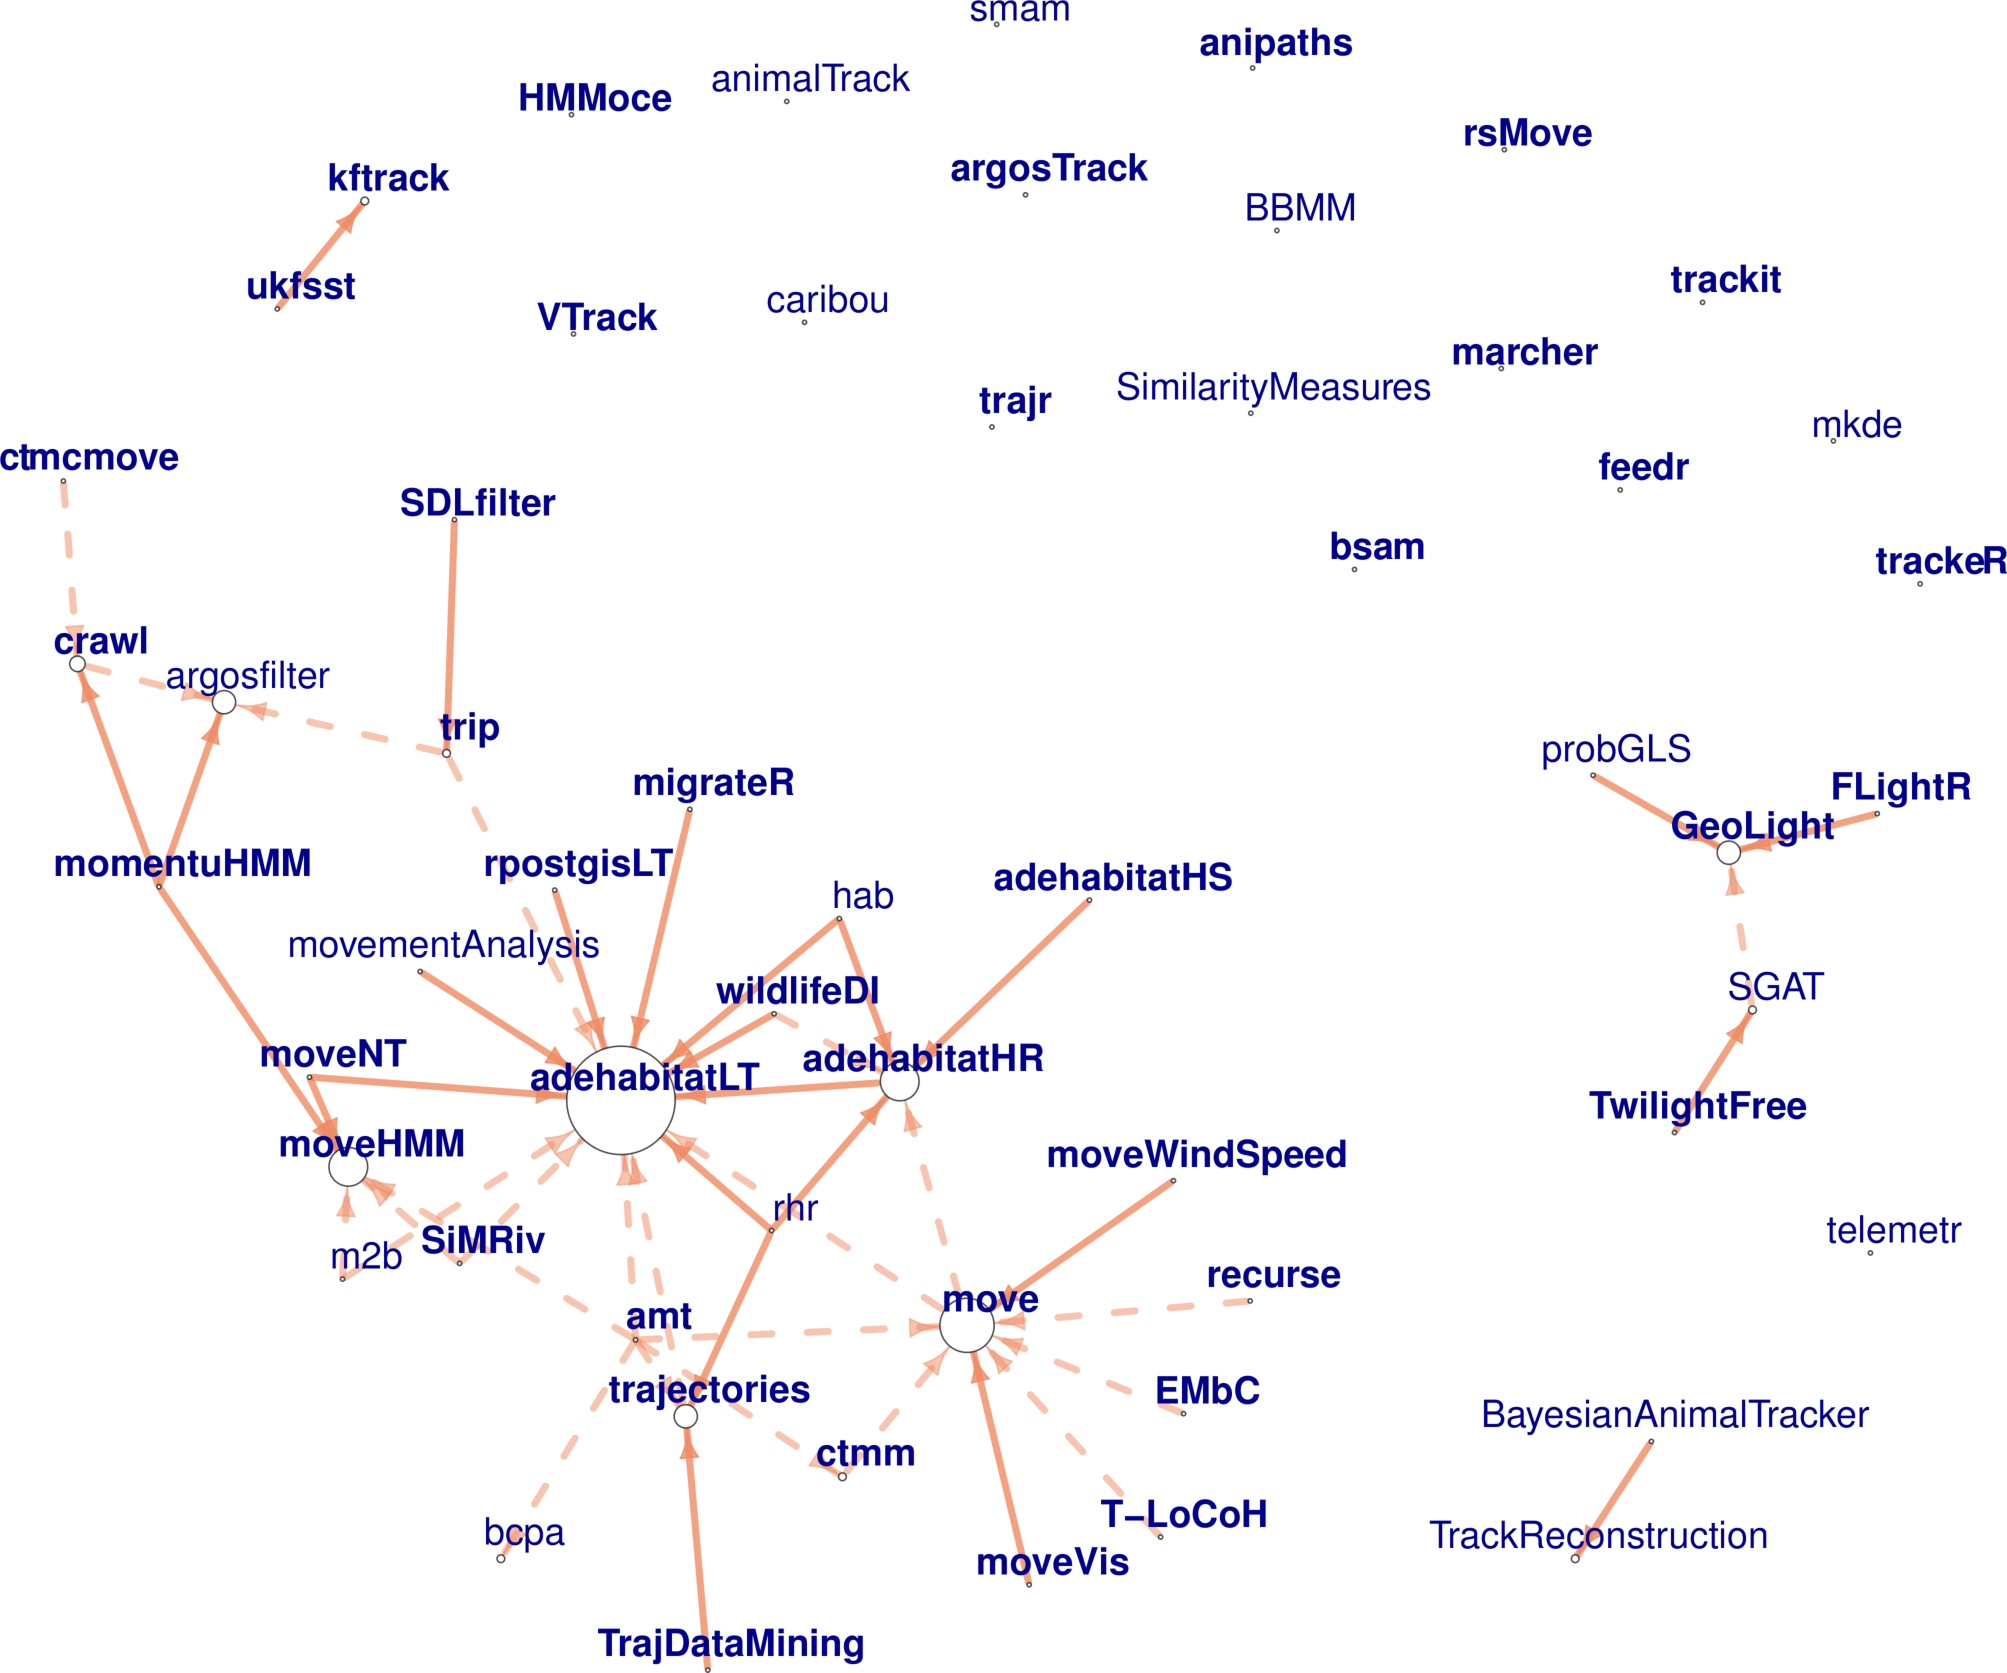
\includegraphics[width=1\textwidth]{./mes_images/NetworkImportSuggestTrack2.pdf}
	\caption{\label{fig:NetImpSuggMov} Network representation of the dependency and suggestion between tracking packages. The arrows go towards the package the others suggest (dashed arrows) or depend on (solid arrows). Bold font corresponds to active packages. The size of the circle is proportional to the number of packages that suggest or depend on this one.}
\end{figure}

\section*{Discussion}
%\label{section:discussion}
%
%I HAVE ADDED SUBHEADINGS, PERHAPS JUST FOR NOW, TO HELP ME VISUALISE THE STRUCTURE
%
\subsection*{Conclusions from the review}

As the quantity and diversity of biologging data increases, so does the need for suitable statistical techniques and software resources. These tools are essential to convert data into ecologically meaningful measures and analyze outputs to test hypotheses. Through a systematic search we identified \textcolor{blue}{57} R packages aimed at processing or analyzing tracking data. The packages offer tools for data processing, visualization, computation of statistics for track description, path reconstruction, behavioral pattern identification, space use characterization and trajectory simulation, among others. 
The main issues for extracting and processing tracking data from biologging devices are already covered by the reviewed packages, and the main types of analyses are covered as well. In some cases, there is more than one package implementing the same type of analysis with the same or very similar approaches, such as \Rpkg{animalTrack} and \Rpkg{TrackReconstruction} for dead-reckoning, \Rpkg{BBMM}, \Rpkg{MovementAnalysis} and \Rpkg{mkde} for Brownian bridge movement models, to cite some examples. Few packages focus on collective motion: mainly \Rpkg{wildlifeDI} and, to a lesser degree, \Rpkg{TrajDataMining} and \Rpkg{movementAnalysis} allow computing descriptive metrics on encounters between individuals, periods of proximity or other metrics of interaction. The lack of tools to analyze collective movement beyond descriptive statistics may be the reflection of a remaining challenge in ecology, and not in computational programming. 
Overall, the review highlighted the abundance and depth of analytical tools available, and identified a need to improve accessibility to existing packages rather than developing new packages.     

\subsection*{Integration over proliferation}

Transparency in science is facilitated by the sharing of data and analysis tools, including code. This has result in a general tendency in the scientific community to convert functions into publicly available packages. In movement ecology, this has translated into a proliferation of R tracking packages, many of them, isolated from the rest (Fig. \ref{fig:NetImpSuggMov}), and with similar goals and methods, as described before. While it is promising that there is a large amount of code available to the scientific community, it is hard to maintain an overview of their functionality and availability. Here we presented a list of \textcolor{blue}{57} packages but the number is expected to keep increasing, with possibilities of task repetitions and disconnected from each other. Due to the already overwhelming number of tracking packages, we suggest developers only create new packages in the future when they represent a substantial contribution to the scientific and programming community. This is difficult to implement however, as package necessity is not assessed through any repository. We recommend future developers reflect on how their package fits into the landscape of current movement ecology packages, in conjunction with users. Methodological journals, which often publish R packages, should ensure that users are involved in the review process and that necessity is a component of the publication decision.

\subsection*{Recommendations}

This work is not intended to tell ecologists exactly which packages to use, but to provide them the catalog of tracking packages, a description of their function and show the similarities and differences between them. We suggest researchers use packages with good documentation, that are actively maintained and that have a large number of users. Good documentation facilitates the initial use of a package, and offers developers an opportunity to link this with pre-existing packages. A regularly maintained package means that there is a person or team behind it, and that, in case of an error in the package, it will likely be fixed rapidly and a new version will be available. A package that has a large number of users means 1) more chances to spot bugs in the package, calling the attention of the maintainer for a rapid repair, and thus making it better and 2) more chances of getting additional guidance on package use from other users. Regarding the methods available in the packages, we previously stated the importance of describing them and citing references. On the other hand, it is the responsibility of the researchers to solely apply a method if they correctly understand it, and not only because it is available in a package. 

When developers are working on new packages, we recommend they consider the following questions:
\begin{itemize}
	\item Does your package fill a gap or need? Does a function of the package perform a novel task that does not already exist in another published package? Can those functions be instead added to an existing package? Developers should contemplate the possibility (and appropriateness) of contacting authors of existing and actively maintained packages to add functions into them. We also suggest the authors of the existing packages to be open to considering the integration of new functions (and new collaborators) to their package.
	\item Does the package handle commonly used data classes (e.g. sp, ltraj), so that it is compatible with the use of other packages?
	\item Is the documentation clear, exhaustive on the functions, with methods description or references available? The latter is even more important if the package implements a new method of analysis. Citing papers rather than explaining the methods is the easiest way to back their procedures up, but authors should consider that not all scientific articles are open access, which means that some potential package users could have free access to the package but not to its methodological support. Worked examples and vignettes can enable researchers to learn the package more easily, minimizing the need for additional support.
	\item Who will maintain the package over time? If a PhD student or a postdoctoral researcher creates a package and after a while is no longer invested in its maintenance, then the lab's PI could take responsibility for the package or delegate responsibility to someone else. 
\end{itemize} 

Taking these questions into account can help maximizing the usefulness of individual packages and strengthen the links between package developers. A stronger community of developers  highly benefits the users: a limited number of strongly-related packages, that are continuously maintained with new functions (and sound documentation) added, are easy to follow and use. Communication between movement ecologists is essential to foster this community. 

\section*{Summary}

The ability to analyze biologging data is essential to answer ecological questions. While the abundance of devices is enabling researchers to collect ever increasing amounts of data, without the necessary tools to interpret this data, their contribution to the field of ecology is unlikely to be realized. Programmers have responded to this need developing up to $57$ R packages, $19\%$ (11) of those in the last year; this review serves as a map of the tools implemented by the packages for data analysis in movement ecology. An increased accessibility and understanding of existing packages will help the advancement of research in this field, allowing researchers to continue to address novel and exciting questions. 
%
%%Avoid repetition. Work together. Even with the human packages. Why not to think about those ones?
%%
%%
%%A stronger community of developers will highly benefit the users: a limited number of strongly-related packages, that are continuously maintained with new functions (and respective documentation) added, are easy to follow and use. Communication between movement ecologist is essential to foster this community
%%
%%Spatial or temporal packages were not part of this review as they are not movement packages. However, they play a major role supporting the movement packages to handle spatiotemporal data. An analysis of package dependency showed that the two most dependent-on packages for movement were sp and raster, two spatial packages (Fig. \ref{fig:DepBarplot}). High in the ranking (with 10 or more dependencies) are also \Rpkg{maptools}, \Rpkg{geosphere}, \Rpkg{rgdal} and \Rpkg{lubridate}, the latter a time related package. A relatively new package that allows handling spatiotemporal data in a simple way is sf (2016). Currently, only \Rpkg{rpostgisLT} and \Rpkg{crawl} depend on this package. Because of its simplicity, sf could be a game changer in R package dependency in the next years: it is expected that new packages will depend on it, and actively maintained movement packages will also have to turn to a sf dependency. \todo[color=blue!20]{Is this paragraph still relevant?}
%%
%%\begin{figure}
%%	\centering
%%	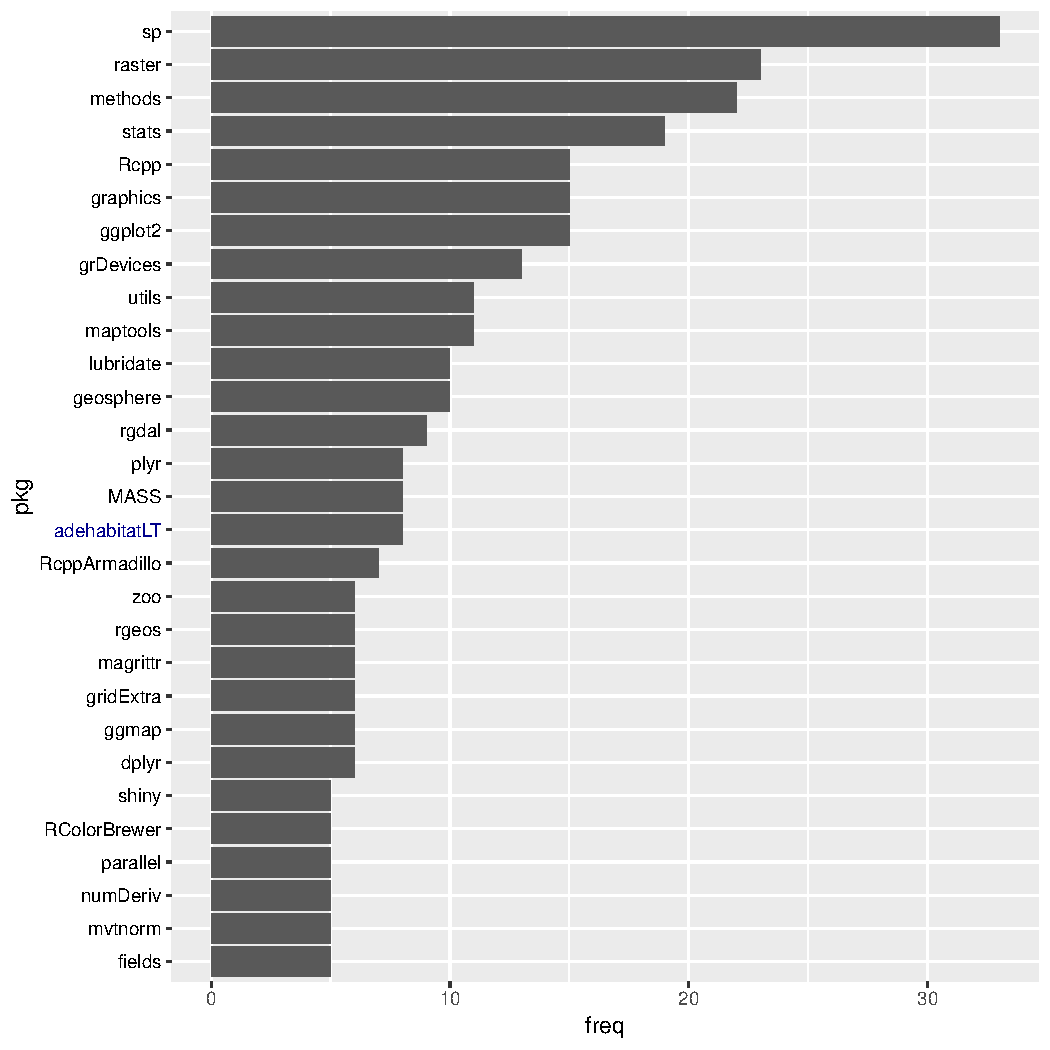
\includegraphics[width=0.75\textwidth]{./mes_images/Dependency-Barplot.pdf}
%%	\caption{\label{fig:DepBarplot} Number of movement packages that require (depend, import or link to) each of these packages. Only the list of packages required by at least 5 movement packages are shown. The text in blue corresponds to a movement package.}
%%\end{figure}
%

\section*{Acknowledgments}

A lot of people are to thank here. HFSP Seabird Sound. Alcohol. So on. 


\newpage


\bibliography{biblio.bib}

%
%\newpage
%
%
%\section*{Tables}
%
%
%\begin{table}[h!]
%  \caption{A first table caption.}
%  \label{Tab1}
%  \begin{center}
%    \begin{tabular}{p{3cm}p{10cm}}
%      Name & Description \\
%      \hline
%      Agri & Proportion of agricultural areas \\
%      Alpine & Proportion of alpine areas \\
%      Bare & Proportion of bare ground \\
%      DEM & Mean elevation \\
%      DEMslope & Mean slope \\
%      \hline
%    \end{tabular}
%  \end{center}
%\end{table}
%
%
%\newpage
%
%
%\begin{table}[h!]
%  \caption{A second table caption, longer than the first one that was
%quite short. Indeed, it was supposed to be short, at the contrary of this one which is
%much more informative than the previous one.}
%  \label{Tab2}
%  \begin{center}
%    \begin{tabular}{lrrr}
%      Name & Mar & Spe1 & Spe2 \\
%      \hline
%      Agri & -0.050 & 0.026 & 0.173 \\
%      Alpine & -0.874 & -0.139 & 0.184 \\
%      Bare & -0.555 & -0.922 & 0.084 \\
%      DEM & -0.796 & -0.100 & 0.095 \\
%      DEMslope & -0.167 & -0.205 & 0.013 \\
%      \hline
%    \end{tabular}
%  \end{center}
%\end{table}
%
%
%\newpage
%
%
%\section*{Figures}
%
%
%\begin{figure}[h!]
%  \caption{What a nice figure\dots}
%  \label{Fig1}
%  \begin{center}
%    \includegraphics[width=6cm]{Fig1}
%  \end{center}
%\end{figure}
%
%
%\newpage
%
%
%\begin{figure}[h!]
%  \caption{Even nicer!}
%  \label{Fig2}
%  \begin{center}
%    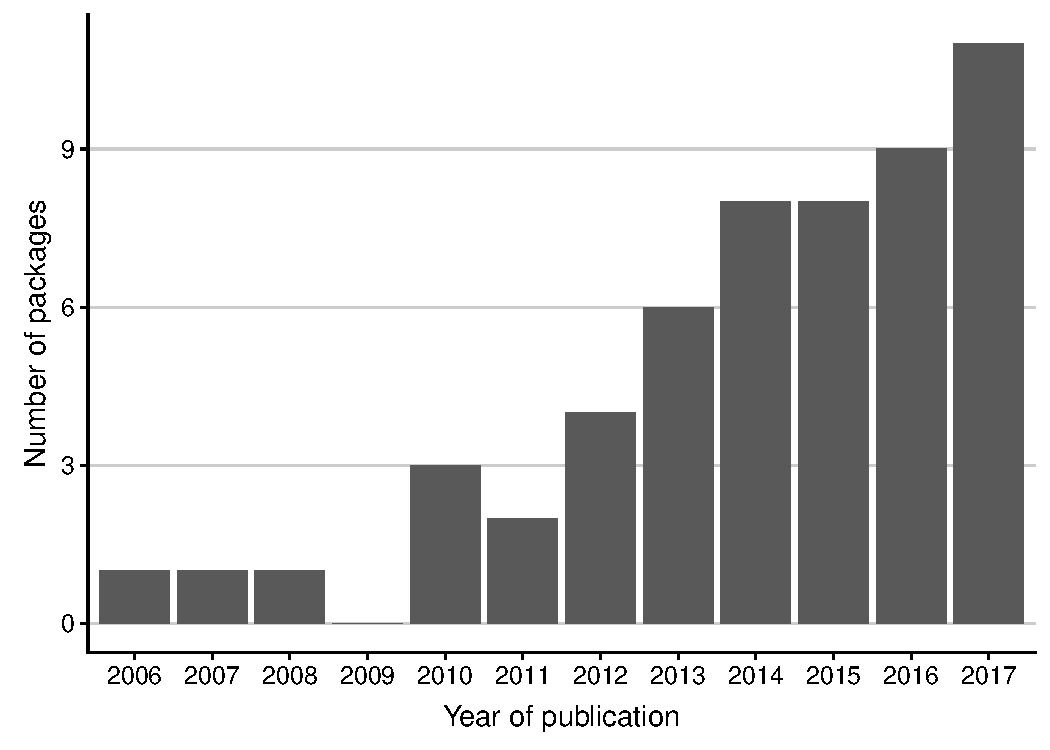
\includegraphics[width=6cm]{Fig2}
%  \end{center}
%\end{figure}


\end{document}
